\documentclass[11pt,letterpaper]{article}
\usepackage[utf8]{inputenc}
\usepackage[margin=1in]{geometry}
\usepackage{graphicx}
\usepackage{hyperref}
\usepackage{booktabs}
\usepackage{enumitem}
\usepackage{xcolor}
\usepackage{float}
\usepackage{listings}

\hypersetup{
  colorlinks=true,
  linkcolor=black,
  urlcolor=blue!60!black,
  citecolor=black
}

\lstset{
  basicstyle=\ttfamily\footnotesize,
  breaklines=true,
  frame=single,
  columns=fullflexible,
  xleftmargin=4pt,
  xrightmargin=4pt,
}

\title{Hurricane Chronicles\\ \large Per-Storm Canvassing Algorithm for Photo and News Archives}
\author{Paul Fishwick and Claude Code}
\date{April 2026}

\begin{document}
\maketitle

\begin{abstract}
Hurricane Chronicles is a Leaflet-based web map that shows a historical hurricane's track across Florida with clickable archive circles at cities along the path. Each circle opens a panel of curated photos and news items drawn from federal, state, and regional archives. A top-bar \emph{MISC} entry holds storm-wide references (Wikipedia, NOAA Monthly Weather Review, interactive web maps) that are not tied to any one city. This document specifies the reusable algorithm that takes a storm track as input and produces populated archive circles as output. The algorithm is tiered: it canvasses cities first at the federal level (Library of Congress), then the state level (University of Florida Digital Collections and Florida Memory), then the regional level (PastPerfect museum catalogs and DPLA). A proximity-based verification step ensures that keyword hits actually describe the storm rather than unrelated content with overlapping vocabulary. A large language model (Claude Opus) is used downstream for bilingual translation and fair-use summarization of fetched pages, but never for URL or citation discovery --- a guardrail motivated by the hallucination incident described in Section~\ref{sec:hallucination}. The 1944 Cuba--Florida Hurricane is the reference implementation; the same recipe applies to any named storm for which a track and date window are known.
\end{abstract}

\tableofcontents
\newpage

%==============================================================================
\section{Goal and Scope}
%==============================================================================

Given a storm identifier, a track (a sequence of \texttt{(lat, lng, time, category)} points), and a date window, the algorithm must output a JSON storm file containing an \texttt{archives} list. Each entry has a city, coordinates, and two lists --- \texttt{news} and \texttt{photos} --- where every item is linkable, captioned, dated, and verifiably about this storm. Figure~\ref{fig:app_overview} shows the rendered result for the 1944 Cuba--Florida Hurricane. The black polyline is the track; the orange dots are populated archive circles ready to be clicked.

\begin{figure}[H]
  \centering
  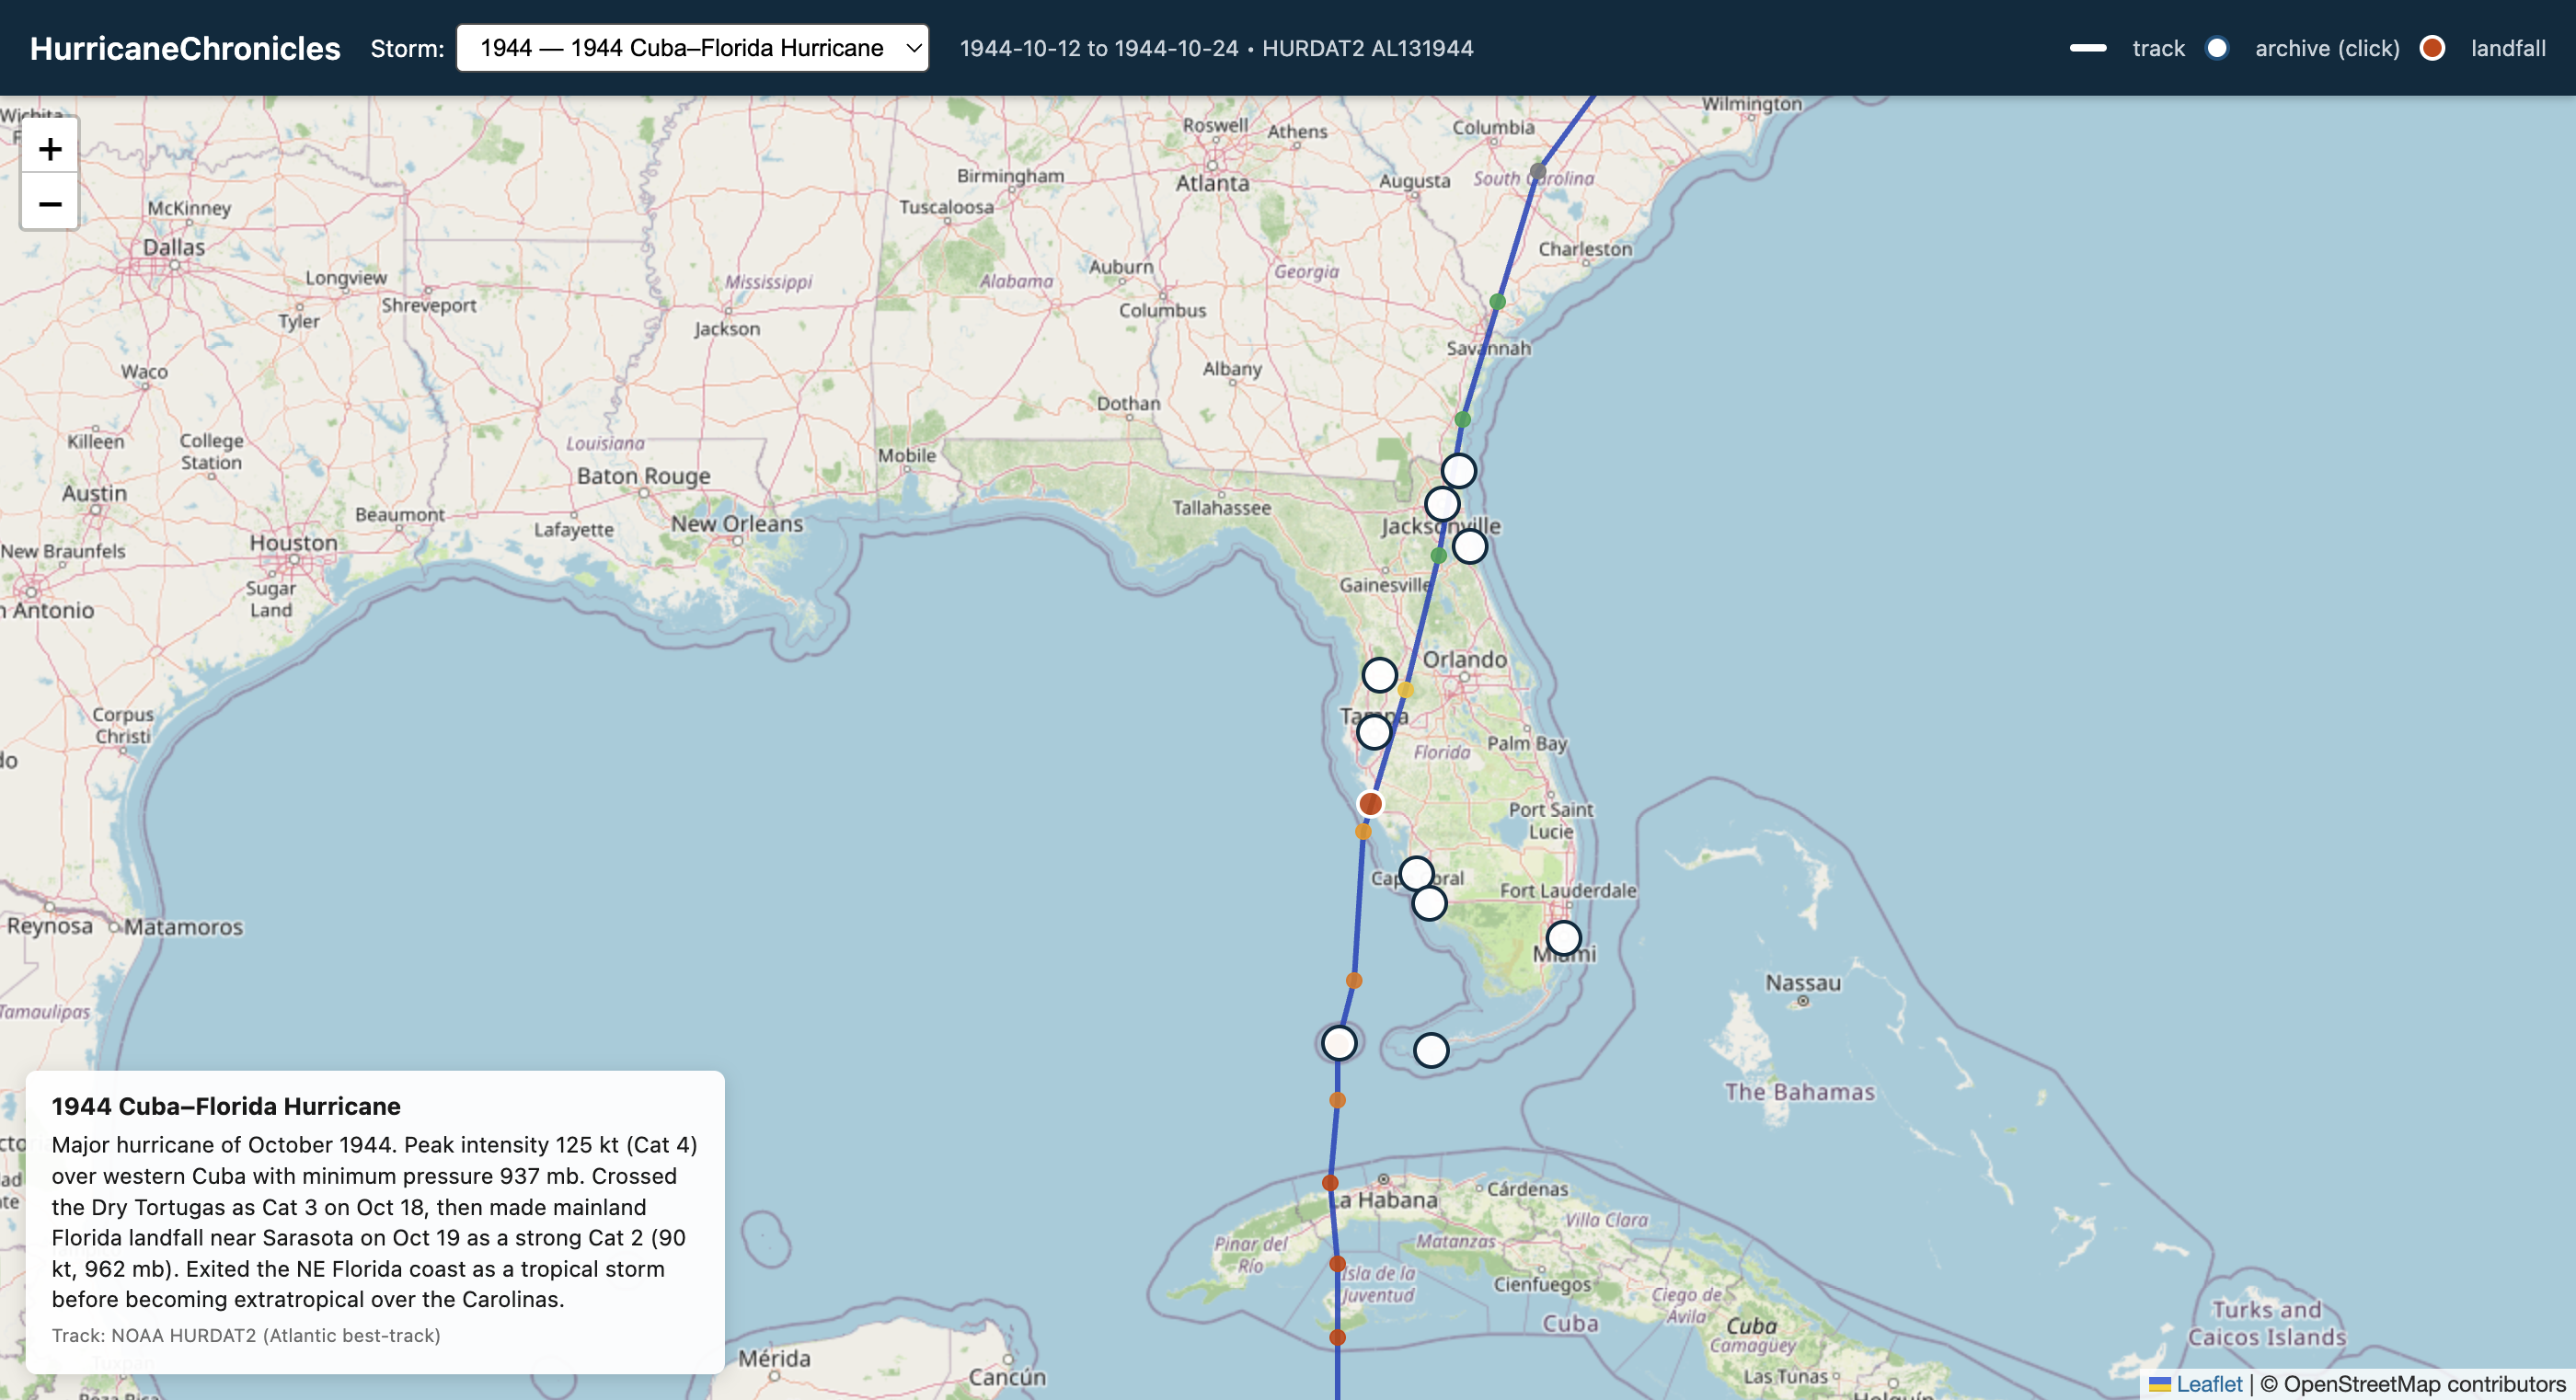
\includegraphics[width=\textwidth]{figures/app_overview.png}
  \caption{Hurricane Chronicles rendering the 1944 Cuba--Florida Hurricane. The track runs from western Cuba across the Dry Tortugas, makes landfall near Sarasota, and exits through northeast Florida. Each orange dot is an archive circle with curated photos and news items.}
  \label{fig:app_overview}
\end{figure}

Three constraints shape the algorithm:

\begin{itemize}
  \item \textbf{Provenance over recall}. Every displayed item must carry an auditable source. A small circle with strong content is preferred to a large one padded with keyword-match noise.
  \item \textbf{Tiered sourcing}. Sources are ranked by reliability, license clarity, and query cost. Federal (LOC) is queried first because it is free, keyword-searchable, and permalinkable. Paid aggregators are excluded.
  \item \textbf{Reusability}. The pipeline must apply unchanged to the next storm with only a new track file and date window. City-specific hand-tuning is minimized.
\end{itemize}

%==============================================================================
\section{Algorithm Overview}
%==============================================================================

The pipeline has six phases. The UML activity diagram is presented in two parts for legibility: Figure~\ref{fig:algorithm_part1} covers discovery (Track $\rightarrow$ Federal $\rightarrow$ State) and Figure~\ref{fig:algorithm_part2} covers the downstream (Regional $\rightarrow$ Verify $\rightarrow$ Render).

\begin{figure}[H]
  \centering
  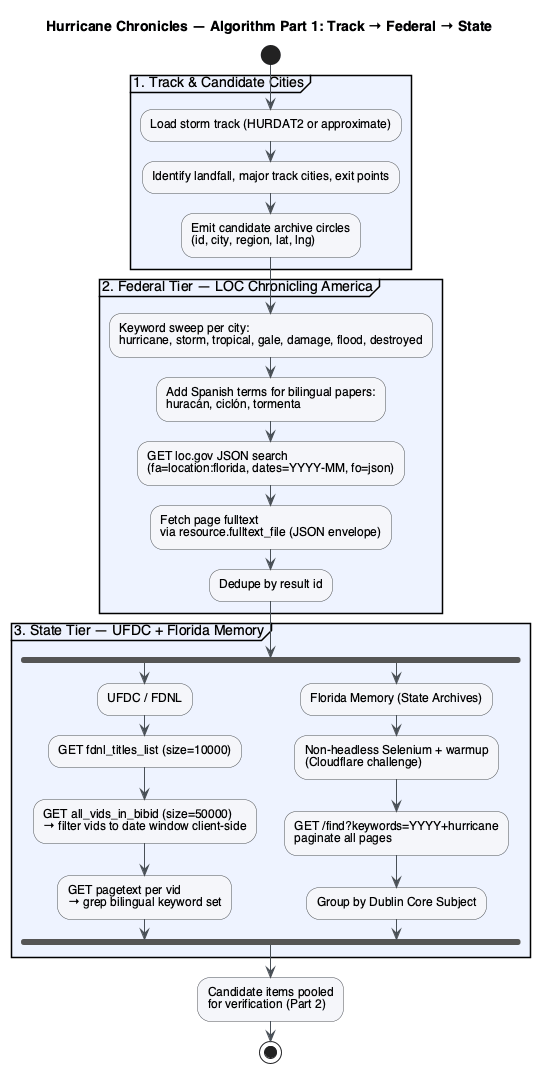
\includegraphics[width=\textwidth,height=0.82\textheight,keepaspectratio]{figures/algorithm_part1.png}
  \caption{Part 1 --- discovery. The fork inside the State tier indicates that UFDC and Florida Memory sweeps run independently. Output is a pool of candidate items passed to Part 2.}
  \label{fig:algorithm_part1}
\end{figure}

\begin{figure}[H]
  \centering
  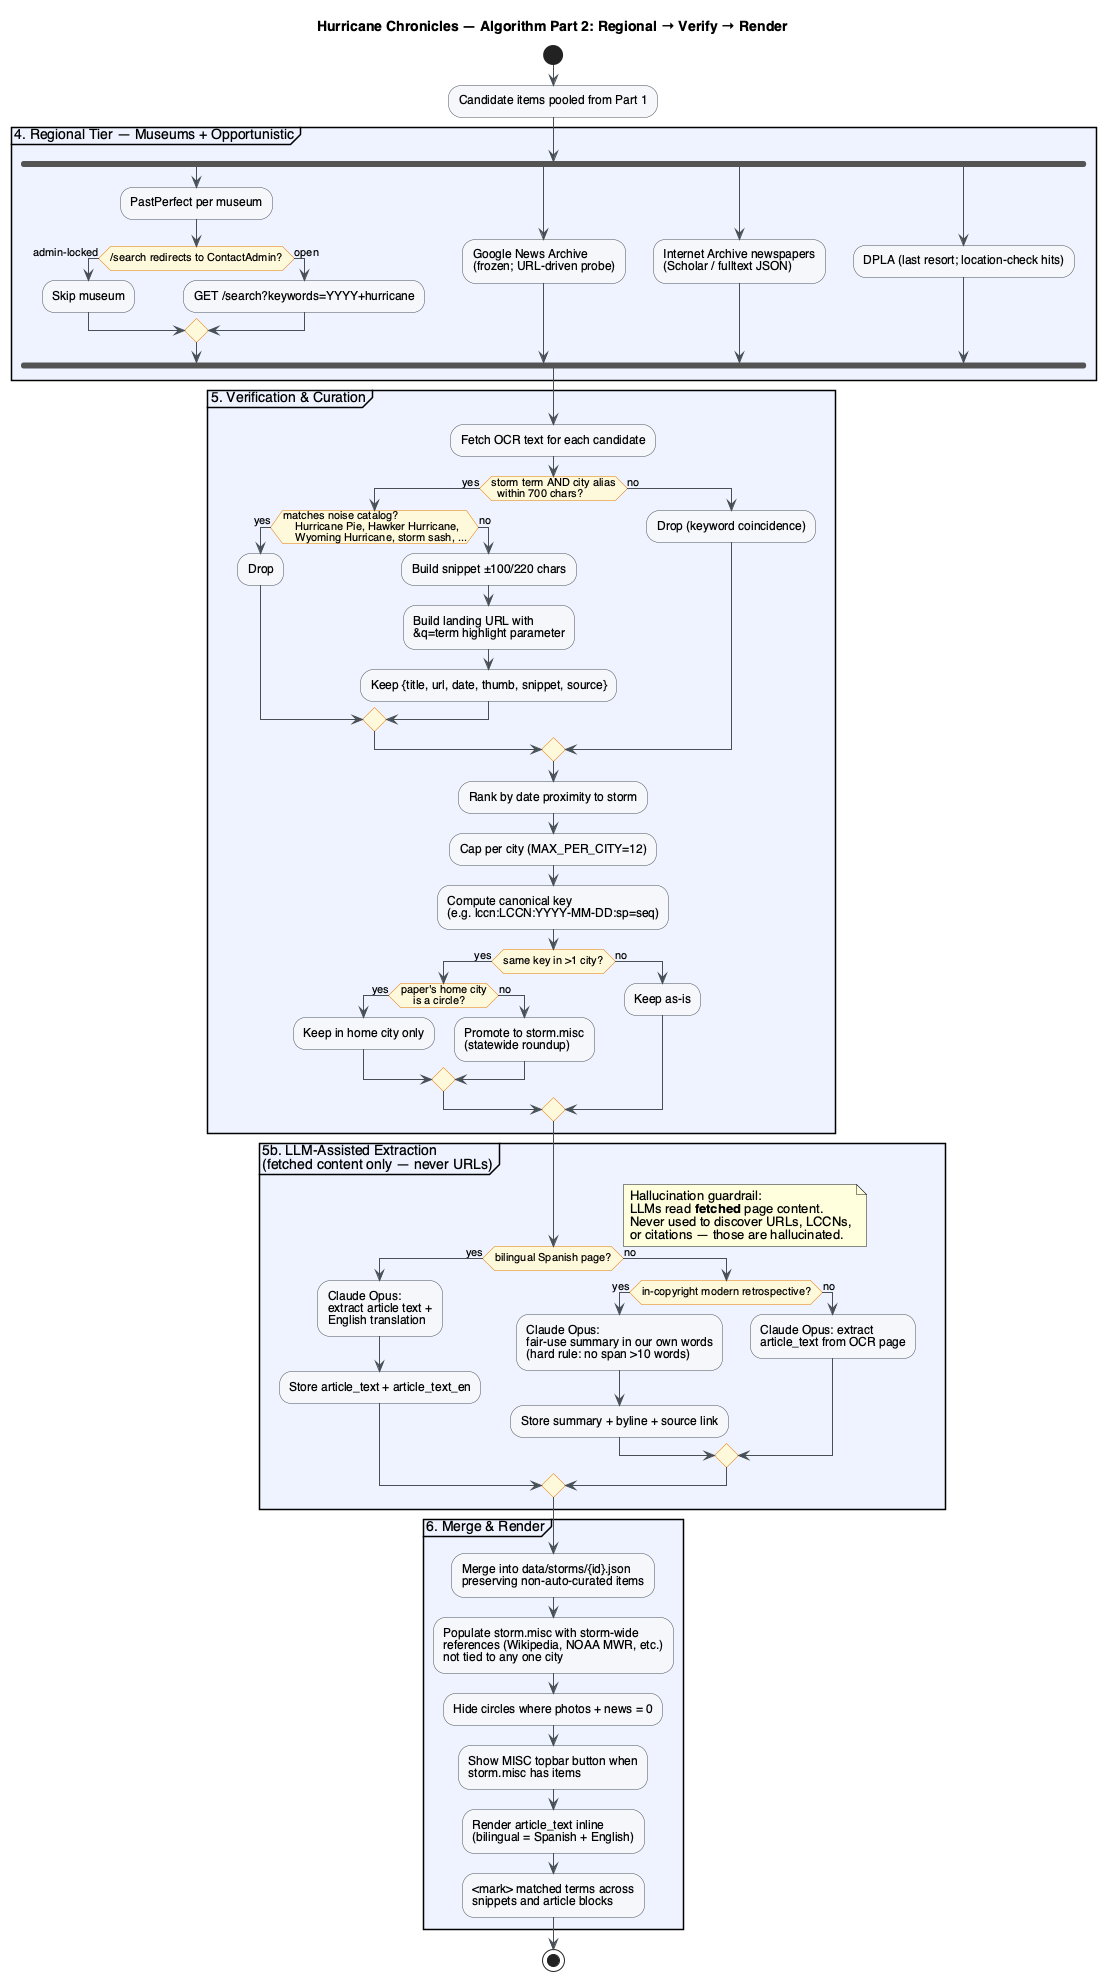
\includegraphics[width=\textwidth,height=0.82\textheight,keepaspectratio]{figures/algorithm_part2.png}
  \caption{Part 2 --- regional sweep (four parallel probes), proximity/noise verification, and rendering. The landing URL is built here with the highlight parameter so the user lands directly on the matched page of the combined viewer.}
  \label{fig:algorithm_part2}
\end{figure}

\newpage
%==============================================================================
\section{Phase 1 --- Track and Candidate Cities}
%==============================================================================

The storm track comes from HURDAT2 where available, or is approximated from historical summaries. Candidate archive circles are chosen by intersecting the track with three classes of locations:

\begin{enumerate}[leftmargin=1.5em]
  \item \textbf{Landfall zones} --- any point where the eye crosses the coast (for the 1944 storm: Dry Tortugas, Sarasota).
  \item \textbf{Major track cities} --- populated places within roughly 60~km of the track line (Key West, Fort~Myers, Tampa, Orlando).
  \item \textbf{Exit points} --- where the storm leaves the state or dissipates (Fernandina Beach).
\end{enumerate}

Each candidate is emitted as a stub: \texttt{\{id, city, region, lat, lng\}}, with empty \texttt{news} and \texttt{photos} lists to be populated downstream.

%==============================================================================
\section{Phase 2 --- Federal Tier: Library of Congress}
%==============================================================================

The Library of Congress Chronicling America collection is the single most important source because it is free, permalinkable, and exposes full-text OCR via JSON. The recipe is given in Listing~\ref{lst:loc}.

\begin{lstlisting}[caption={LOC Chronicling America query pattern},label=lst:loc]
GET https://www.loc.gov/search/
    ?q=<keyword>
    &fa=partof:chronicling+america|location:florida
    &dates=YYYY-MM/YYYY-MM
    &fo=json&c=40
--> results[].id       # permalink to the page viewer
--> results[].date     # publication date
GET <result.id>&fo=json
--> resource.fulltext_file
GET <fulltext_file>    # JSON envelope, NOT XML despite the alto_xml URL
--> body.full_text     # 10-25 KB of OCR text
\end{lstlisting}

Three properties of this endpoint drive the design:

\begin{itemize}
  \item \textbf{Keyword breadth matters.} A single query for \emph{hurricane} finds only a fraction of real storm coverage. Broaden to \{\emph{hurricane}, \emph{storm}, \emph{tropical}, \emph{gale}, \emph{damage}, \emph{flood}, \emph{destroyed}\} and deduplicate by result \texttt{id}.
  \item \textbf{Spanish-language papers exist.} La Gaceta (Tampa) and parts of the Miami press are bilingual. English \emph{hurricane} returns zero hits for La Gaceta in October 1944; Spanish \{\emph{hurac\'an}, \emph{cicl\'on}, \emph{tormenta}\} returns coverage in eleven of thirteen issues in the window.
  \item \textbf{Cloudflare protects loc.gov.} Plain \texttt{urllib} gets 403. The project uses non-headless Selenium with \texttt{--disable-blink-features=AutomationControlled}; the JavaScript challenge clears in about one second with no user interaction.
\end{itemize}

The legacy endpoint \texttt{chroniclingamerica.loc.gov/.../ocr.txt} is dead (permanent 403 after a Cloudflare redirect). Only the new \texttt{www.loc.gov} JSON endpoints work.

%==============================================================================
\section{Phase 3 --- State Tier: UFDC and Florida Memory}
%==============================================================================

The state tier runs in parallel with two independent sweeps.

\subsection{UFDC / Florida Digital Newspaper Library}

UFDC (hosted by the University of Florida) fills the major gap in LOC's Florida coverage --- the big-city dailies (Tampa Tribune, Sarasota Herald-Tribune, Fort~Myers News-Press, Orlando Sentinel, Jacksonville Times-Union, Miami Herald in partial runs). Its JSON API at \texttt{api.patron.uflib.ufl.edu} is free and unauthenticated:

\begin{lstlisting}[caption={UFDC two-step query}]
GET /fdnl_titles_list?size=10000
  --> filter bibids where min_date <= storm_year <= max_date
GET /all_vids_in_bibid?bibid=<X>&size=50000   # NOT the default 1000!
  --> filter vids client-side to the storm's date window
GET /pagetext?bibid=<X>&vid=<Y>
  --> hits[{pagetext, pageorder, thumbnail}]
\end{lstlisting}

Two UFDC-specific traps are worth calling out. First, the \texttt{publication\_date} query parameter performs token matching, not range filtering --- a query for \texttt{1944-10-12 TO 1944-10-26} returns 1920s issues mixed in. Always filter dates client-side. Second, the default \texttt{size} on \texttt{all\_vids\_in\_bibid} is 1000; La Gaceta has over 12000 issues, so the default truncates before reaching 1944. Always pass \texttt{size=50000}.

\subsection{Florida Memory (State Archives of Florida)}

Florida Memory is the State Archives' photographic collection --- Dublin-Core catalogued, richly captioned, and the only source for many small-town 1944 hurricane photographs. It is behind Cloudflare and actively blocks headless browsers.

\begin{itemize}
  \item Use \emph{non-headless} Selenium with \texttt{--disable-blink-features=AutomationControlled}.
  \item \textbf{Warmup}: visit a known-good \texttt{/items/show/<id>} page first so Cloudflare issues cookies, then proceed to search.
  \item Query \texttt{/find?keywords=YYYY+hurricane} and paginate. City-specific variants (\texttt{hurricane+Tampa+1944}) added zero new items for the 1944 storm --- the generic query returns everything.
  \item Group hits into circles by parsing the Dublin Core \texttt{Subject} tag (\texttt{Hurricanes--Florida--<County>--<City>}).
\end{itemize}

%==============================================================================
\section{Phase 4 --- Regional Tier: PastPerfect and DPLA}
%==============================================================================

\subsection{PastPerfect Online}
Many small Florida museums publish catalogs on PastPerfect at URLs of the form \texttt{\{museum\}.pastperfectonline.com}. Coverage is uneven: some museums leave search fully open, others have disabled it and redirect \texttt{/search} to \texttt{/Home/ContactAdmin}. The canvassing script probes each candidate and aborts that museum on the redirect. For the 1944 reference storm, only the Amelia Island Museum of History yielded useful results (eighteen photos).

\subsection{DPLA}
DPLA aggregates US archives but is used only as a last resort. It excludes Florida State Archives (Florida Memory), and location sanity-checking is mandatory --- a search for \emph{Arlington hurricane 1944} will happily return items from Arlington, Massachusetts mis-grouped under the Florida circle.

\subsection{Google News Archive}
Google's newspaper archive (\texttt{news.google.com/newspapers}) has been frozen since 2011 but remains viewable and holds a usable set of Florida dailies, notably the \emph{St.~Petersburg Times} and \emph{Evening Independent} with searchable 1940s issues. No official API exists. Probing is URL-driven: a search of the form \texttt{news.google.com/newspapers?nid=\{paper-id\}\&dat=YYYYMMDD} returns an image viewer with OCR overlay. The project treats this source as opportunistic --- low yield, zero cost, fragile against any Google-side change. If Google removes the archive (repeatedly rumoured since 2011), no code in the pipeline depends on it.

\subsection{Internet Archive newspapers}
\texttt{archive.org/details/newspapers} hosts a growing set of uploaded historical newspapers with full-text OCR. 1940s Florida coverage is sparse but not zero, and the query path is clean: the Scholar and fulltext APIs return JSON. This source is checked last in the regional tier and pooled with PastPerfect hits before the verification step. Items must carry an \texttt{archive.org} source tag so readers can distinguish them from institutional holdings.

\subsection{What is deliberately out of scope}
\textbf{Newspapers.com} holds the largest Florida dailies but is a paid service with terms-of-service restrictions that preclude automated scraping. \textbf{ProQuest Historical Newspapers} has the deep \emph{Miami Herald} run but is institution-gated. \textbf{NewsBank / GenealogyBank / HathiTrust} each hold partial FL content but either require subscription or (for HathiTrust) restrict in-copyright material. These are noted only so future contributors know why obvious-looking sources are absent.

%==============================================================================
\section{Phase 5 --- Verification and Curation}
%==============================================================================

Keyword matching alone produces unacceptable noise: roughly half of 1944 \emph{hurricane} hits in LOC are false positives (see the Appendix). Every candidate item is verified by a proximity rule before it is kept.

\paragraph{Proximity rule.} Given the OCR text, an item is accepted only if a storm term and a city alias both appear, and their character positions are within \texttt{PROXIMITY=700} characters of each other --- tight enough to mean ``same article,'' loose enough to allow for column breaks and ad insertions. The snippet emitted into the UI spans roughly 100 characters before to 220 after the closer match. The reference implementation is \texttt{find\_snippet()} in \texttt{tests/auto/curate\_news.py:118}.

\paragraph{Noise filtering.} Hits that match the catalog of known false positives (Appendix~A) are dropped before the proximity rule is even applied. This catalog grows with each new storm; additions should be code-reviewed because they are effectively project-wide denylists.

\paragraph{Ranking and cap.} Kept items are ranked by date proximity to the storm (storm-month best, month+1 second, later worse) and capped at \texttt{MAX\_PER\_CITY=12}. The cap prevents a single verbose paper from dominating a circle.

\paragraph{Cross-city dedupe and the home-paper rule.} A proximity-verified candidate can legitimately match several cities at once: a small-circulation weekly that ran a statewide storm roundup will mention Tampa, Sarasota, Jacksonville, and Orlando on the same page, and the per-city curation loop will naively place that single page into four different circles. The pipeline therefore computes a canonical key per candidate --- for LOC items, \texttt{lccn:\{LCCN\}:\{YYYY-MM-DD\}:sp=\{seq\}} --- and enforces that each key appears at most once across the merged output. When a key would land in more than one city, the \emph{home-paper rule} applies: if the paper's home city is itself a circle (e.g.\ \emph{The Brooksville Journal} for Brooksville), the item stays there; otherwise it is promoted to \texttt{storm.misc.news} as a statewide reference. This is how \emph{Gadsden County Times} (Quincy, NW Florida --- no circle on this storm's track) arrived in MISC, while \emph{Brooksville Journal} issues stayed in the Brooksville circle. The effect: newspaper sources whose coverage is intrinsically statewide show up exactly once, in the bucket where they carry the most signal.

%==============================================================================
\section{Landing URLs --- Always Text + Image + Highlight}
%==============================================================================

Every curated news item carries a \texttt{url} field. This URL is where the user lands when they click the item in the side panel. The project's standing rule is: \emph{when the source archive offers a combined text-and-image viewer, link there --- never to a text-only or image-only fallback, and always with the matched term as a highlight parameter}. Table~\ref{tab:viewers} gives the deep-link pattern per source.

\begin{table}[H]
\centering
\small
\begin{tabular}{@{}p{3.2cm}p{1.6cm}p{1.6cm}p{1.6cm}p{5.6cm}@{}}
\toprule
\textbf{Source} & \textbf{Image} & \textbf{OCR text} & \textbf{Highlight} & \textbf{Landing URL pattern} \\
\midrule
LOC Chronicling America & yes & yes & yes & \texttt{\{result.id\}?q=\{term\}} \\
UFDC / FDNL & yes & yes & yes & \texttt{ufdc.ufl.edu/\{bibid\}/\{vid\}/\{pageorder\}?qs=\{term\}} \\
Google News Archive & yes & overlay & partial & \texttt{news.google.com/newspapers?nid=\{id\}\&dat=\{YYYYMMDD\}} \\
Internet Archive & yes & yes & yes & \texttt{archive.org/details/\{id\}/page/\{n\}/mode/2up?q=\{term\}} \\
Florida Memory (photos) & yes & caption only & n/a & \texttt{floridamemory.com/items/show/\{id\}} \\
PastPerfect & thumbnail & caption only & n/a & museum-specific \texttt{/Detail/.../\{id\}} \\
\bottomrule
\end{tabular}
\caption{Deep-link pattern per source. Columns indicate whether the landed-on page shows the scanned image, the OCR text, and a visible highlight of the matched term. Newspaper sources always support all three; photo/catalogue sources land on the item page with its own caption metadata.}
\label{tab:viewers}
\end{table}

Three consequences follow from this rule:

\begin{itemize}[leftmargin=1.5em]
  \item \textbf{No bare PDFs.} Even when a source provides a PDF download, the \texttt{url} points to the viewer, not the PDF --- users need the OCR highlight to locate the story on the page.
  \item \textbf{Store the page, not the issue.} The viewer URL must deep-link to the specific page (\texttt{pageorder}, \texttt{sp}, or equivalent). Landing users on issue covers wastes their time.
  \item \textbf{If a source lacks a combined viewer, downgrade it.} If the only available URL shows image-without-text or text-without-image, that source drops to the regional tier and the snippet in the panel must stand in for the missing view. Google News Archive is in this category --- its OCR overlay is partial, so the panel snippet from our own OCR grep is what carries the reader.
\end{itemize}

The reference implementation constructs the LOC URL at \texttt{curate\_news.py:225--226}. Equivalent URL builders for UFDC and Internet Archive should mirror that pattern: append the match term as a highlight parameter rather than pointing at a raw page.

%==============================================================================
\section{Phase 6 --- Merge and Render}
%==============================================================================

Curated items are merged back into \texttt{data/storms/\{id\}.json}, preserving any hand-curated entries not sourced from the tiered pipeline. Two UI rules close the loop:

\begin{enumerate}[leftmargin=1.5em]
  \item \textbf{Hide empty circles.} \texttt{renderArchives()} filters \texttt{a => a.photos.length + a.news.length > 0}. This keeps the storm track implicit in the populated circles and avoids inviting clicks that produce empty panels.
  \item \textbf{Highlight matched terms.} News snippets wrap the matched terms (\emph{hurricane}, \emph{hurac\'an}, \emph{cicl\'on}, \emph{storm}, \emph{tormenta}, \emph{damage}, \emph{tropical}, \emph{flood}, \emph{gale}, \emph{destroyed}) in \texttt{<mark>} so readers do not have to skim walls of OCR.
\end{enumerate}

\subsection{Inline article extraction and bilingual rendering}

For news items whose underlying source exposes OCR text, the pipeline runs a post-curation extraction pass (\texttt{tests/auto/widen\_translate\_all.py}) that fetches the page text and stores it directly in the item as \texttt{article\_text}. The panel then renders that text in place, so a visitor never has to click out to a PDF viewer to read the story. The specific patterns are:

\begin{itemize}[leftmargin=1.5em]
  \item \textbf{English-only OCR.} The pipeline stores the full page text in \texttt{article\_text}; the panel shows it inline with yellow \texttt{<mark>} highlighting on the same keyword set used during verification, followed by a ``View original page $\rightarrow$'' link to the archive's combined image+text viewer.
  \item \textbf{Bilingual pages (Spanish originals).} For \emph{La Gaceta} (Tampa) and similar bilingual papers, Claude Opus is invoked on the \emph{fetched} page text to produce an English translation. Both are stored (\texttt{article\_text}, \texttt{article\_text\_en}), and the panel renders them stacked: a purple-accented ``Original (Spanish)'' block followed by a green-accented ``English translation'' block, with the yellow highlight applied to both. Visitors who do not read Spanish can still follow the coverage end-to-end in the panel.
  \item \textbf{In-copyright modern retrospectives.} Some of the best context is in modern newspaper retrospectives (e.g.\ \emph{The St.\ Augustine Record}, 2010) that cannot be reproduced verbatim. The pipeline (\texttt{tests/auto/fetch\_retrospective.py}) fetches the page, passes it to Claude Opus with a hard rule that no quoted span may exceed $\sim$10 consecutive words, and stores a two- to three-sentence summary under \texttt{summary} together with \texttt{byline} and \texttt{source}. The panel renders this as a purple ``Summary (our words)'' card with a prominent ``Read the full story at \emph{source} $\rightarrow$'' link. Fair-use, link-forward.
\end{itemize}

\subsection{Storm-wide references: the MISC bucket}

Some material is about the storm itself, not about any single city along the track: the Wikipedia article on the storm, the Wikipedia season overview, the NOAA Monthly Weather Review PDF, Esri/ArcGIS StoryMaps web maps, and similar. Forcing these into a specific city circle would be misleading. The schema therefore supports a sibling block to \texttt{archives} at the storm level:

\begin{lstlisting}[caption={Storm-wide references block}]
{
  "hurdat_id": "AL131944",
  "name": "1944 Cuba-Florida Hurricane",
  ...
  "archives": [ ... per-city photos/news ... ],
  "misc": {
    "photos": [ ],
    "news":   [ { kind, title, url, source, date, description } ]
  }
}
\end{lstlisting}

When \texttt{storm.misc} contains any items, the UI shows a \texttt{MISC} button in the top bar next to the HURDAT2 metadata. Clicking it opens the same archive panel used by city circles, but with the synthetic title ``Miscellaneous'' and subtitle ``\{storm name\} --- storm-wide references.'' Two new \texttt{kind} values were introduced for this bucket: \texttt{encyclopedia} (Wikipedia articles) and \texttt{primary-document} (NOAA MWR, U.S. Weather Bureau reports). The existing \texttt{retrospective} kind is reused for StoryMaps and similar narrated overviews. Storms without a \texttt{misc} block hide the button automatically; no UI change is required between storms.

%==============================================================================
\section{Hallucination Mitigation}
\label{sec:hallucination}
%==============================================================================

Large language models are used in several places in this pipeline --- for bilingual translation, fair-use retrospective summarization, and keyword/noise judgment during candidate verification. Early in development we also experimented with using an LLM-backed web search API (Perplexity Sonar, routed through OpenRouter) as a \emph{discovery} tool: given a broad natural-language query, return a ranked list of candidate URLs across federal, state, and regional archives. This subsection documents why that experiment was abandoned and what guardrail replaced it.

\subsection{The Palatka incident}

During a multi-query Sonar discovery run against the 1944 Cuba--Florida Hurricane, the service returned the following plausible-looking citation:

\begin{lstlisting}[caption={The hallucinated citation}]
title:  "Palatka Daily News - October 19, 1944 (hurricane coverage)"
url:    https://www.loc.gov/resource/sn95047260/1944-10-19/ed-1/?sp=1
source: "The Palatka Daily News - LOC Chronicling America"
\end{lstlisting}

Every surface feature of this record was correct:

\begin{itemize}[leftmargin=1.5em]
  \item URL shape matched the \texttt{www.loc.gov/resource/\{lccn\}/\{date\}/ed-\{n\}/} form used throughout Phase 2.
  \item Date (\texttt{1944-10-19}) fell squarely inside the storm window.
  \item LCCN had the correct Chronicling America serial-number format (\texttt{sn\#\#\#\#\#\#\#\#}).
  \item City (Palatka) is a real St.\ Johns River town near the storm track.
  \item Paper name (\emph{Palatka Daily News}) is a real, historically-digitized paper.
\end{itemize}

A direct fetch against the URL, however, returned 404. Resolving the LCCN at \texttt{loc.gov/item/sn95047260/?fo=json} showed it actually belongs to \emph{The Sun} (Belle Glade, Fla.), 1989--2018 --- wrong paper, wrong decade, wrong half of the state. A separate LOC title search confirmed that \emph{no} Palatka newspaper covering the 1940s is digitized in Chronicling America at all: the real \emph{Palatka Daily News} (LCCN \texttt{sn78001466}) ends at 1922.

The citation had passed every plausibility filter the pipeline applies: primary-archive domain, correct URL template, correct date, real city, real paper name. What it failed was the one check that cost a network request: actually fetching the page.

\subsection{Why LLMs cannot be trusted for citation discovery}

The failure is not an isolated bug. LLMs compose responses from statistical patterns over training text, and archive citations are exactly the kind of structured, pattern-regular content where fluent-looking hallucinations are most likely and hardest to detect from the surface alone. An LCCN is eight digits after \texttt{sn}; a Chronicling America URL follows a rigid template; a hurricane-coverage page is expected to exist in any major Florida paper's October 1944 run. The model has strong priors for all of these, and will happily emit a syntactically valid permalink that references a paper that was never digitized, or a date on which no edition exists.

Compounding the problem, the hallucination rate appears low enough that batch triage gives false confidence. In the 1944 discovery run, one fabricated LCCN was enough to corrupt an ingest: once the Palatka entry was added, verifying the remaining 84 ``primary-archive'' leads manually would have been required before any of them could be trusted --- which defeats the purpose of having the LLM surface them in the first place.

\subsection{The guardrail: fetch-before-trust, never LLM-discovered URLs}

The project rule is now:

\begin{itemize}[leftmargin=1.5em]
  \item \textbf{LLMs may read fetched content; they may not discover URLs.} Translation, summarization, and noise-catalog judgment all operate on bytes returned by a real HTTP request. No step in the pipeline accepts a URL, LCCN, bibid, or image ID that was generated by an LLM.
  \item \textbf{Discovery uses built-in web search.} For broad discovery, the project uses Claude Code's native \texttt{WebSearch} tool (which backs onto real Google/Bing results), not an LLM-synthesized citation list. Results are real search hits from real crawlers; the model is not inventing URLs.
  \item \textbf{Every candidate URL is fetch-tested before ingest.} The candidate verification step that used to check OCR proximity now also verifies that the URL resolves, that the returned page's content matches the claimed title/date, and for LOC specifically, that the LCCN resolves at \texttt{loc.gov/item/\{lccn\}/?fo=json} to a paper whose \texttt{dates\_of\_publication} span the target year.
  \item \textbf{Rollback hurt, but rollback was easy.} The Palatka entry was removed by deleting one archive dict from the storm JSON. This argues for keeping the schema flat and idempotent: no cross-references, no derived aggregates, so a bad ingest can be undone without surgery.
\end{itemize}

The constraint that LLMs read fetched content only --- illustrated as a \emph{note} on Step 5b of the Part 2 flowchart (Figure~\ref{fig:algorithm_part2}) --- is the single most important addition to the pipeline since the original design, and applies to any future LLM the project adopts.

%==============================================================================
\section{Reusable Recipe for the Next Storm}
%==============================================================================

To apply this pipeline to a new storm, the inputs are (a) the track, (b) the storm date window (roughly one week before landfall through three weeks after), and (c) the list of candidate cities from Phase~1. Then:

\begin{enumerate}[leftmargin=1.5em]
  \item Write \texttt{data/storms/\{id\}.json} with the track and empty archive stubs.
  \item Add the \texttt{id} to \texttt{data/storms.json}.
  \item Run the LOC sweep (\texttt{tests/auto/curate\_news.py}) against the new date window.
  \item Run the UFDC sweep (analogous script, same API, same filters).
  \item Run the Florida Memory sweep with the generic \texttt{YYYY+hurricane} keyword.
  \item Probe PastPerfect per candidate museum; keep only the open ones.
  \item Treat DPLA as optional. If used, location-check every hit.
  \item Apply the proximity rule and noise catalog.
  \item Run \texttt{widen\_translate\_all.py} to extract \texttt{article\_text} for each kept news item (with English translation if the source is Spanish).
  \item If modern in-copyright retrospectives are worth linking, run \texttt{fetch\_retrospective.py} to produce fair-use summaries.
  \item Populate \texttt{storm.misc} with storm-wide references (Wikipedia article, NOAA MWR PDF, StoryMap). \textbf{Verify every candidate URL with a real HTTP fetch before adding it} (see Section~\ref{sec:hallucination}).
  \item Merge, verify visually in the browser, and commit.
\end{enumerate}

No code in \texttt{js/app.js} should need to change between storms. If it does, the storm schema has been violated.

%==============================================================================
\appendix
\section{Noise Catalog (False Positives)}
%==============================================================================

Recurring false positives observed during the 1944 curation:

\begin{itemize}[leftmargin=1.5em]
  \item \textbf{``Hurricane Pie''} --- a WWII recipe column using apple windfalls.
  \item \textbf{``Wyoming Hurricane''} --- a 1944 Russell Hayden cowboy film.
  \item \textbf{``Summer Storm''} --- a 1944 Linda Darnell film.
  \item \textbf{``Hawker Hurricane'' / ``Spitfire and Hurricane''} --- RAF fighter planes, ubiquitous in WWII news.
  \item \textbf{``Hurricane lamp''} --- classified ads.
  \item \textbf{``Storm troops''} --- political metaphor for Nazi brownshirts.
  \item \textbf{``Storm sash''} --- building-supplies ads.
  \item \textbf{``Storm in Connecticut''} --- agriculture news from other states.
\end{itemize}

%==============================================================================
\section{Keyword Sets}
%==============================================================================

\noindent\textbf{English}: \emph{hurricane, storm, tropical, gale, damage, flood, destroyed}.\\
\noindent\textbf{Spanish} (Tampa and Miami bilingual papers): \emph{hurac\'an, cicl\'on, tormenta}.\\
\noindent\textbf{City aliases}: always include the common shortened form (\emph{St.~Pete} for St.~Petersburg), the historic name where relevant (\emph{Estero} for the Fort~Myers Beach area in 1944), and the nearest-large-city fallback (\emph{Key West} as a proxy for \emph{Dry Tortugas}, which almost never appears in headlines).

%==============================================================================
\section{Source Matrix}
%==============================================================================

\begin{table}[H]
\centering
\small
\begin{tabular}{@{}p{3.2cm}p{2.2cm}p{4.2cm}p{4.8cm}@{}}
\toprule
\textbf{Source} & \textbf{Tier} & \textbf{Content} & \textbf{Access note} \\
\midrule
LOC Chronicling America & Federal & Small-paper newspaper OCR & Cloudflare; use Selenium JSON fetch \\
UFDC / FDNL & State & Major FL dailies full-text & Free JSON API; client-side date filter \\
Florida Memory & State & Photos, postcards, audio & Non-headless Selenium with warmup \\
PastPerfect Online & Regional & Museum catalogs & Per-museum; many admin-locked \\
Google News Archive & Regional & Frozen FL dailies (St.~Pete, etc.) & URL-driven; opportunistic, fragile \\
Internet Archive News & Regional & Sparse uploaded papers & Scholar / fulltext API; JSON \\
DPLA & Aggregator & Cross-archive items & Last resort; location-check required \\
Newspapers.com, ProQuest, HathiTrust, NewsBank & (excluded) & Major FL dailies & Paid / institution-gated \\
\bottomrule
\end{tabular}
\caption{Archive sources by tier with access characteristics.}
\label{tab:sources}
\end{table}

\end{document}
